\chapter{Introduction to Probability}
The concept ``probability'' is used very often in everyday language to describe the chance of something happening. Mathematically, Probability is a language to quantify uncertainty. 
This chapter will introduce necessary and basic concepts and namely, \textbf{Probability Theory}. We will start the chapter about interpretations of probability. \\
We will introduce the concepts fast. since they are rather easy compared to next chapters.
%-------------------------------------------------
\section*{Discrete Versus Continuous Concepts}
Before we even begin with our concepts. we must learn the difference between the terms \textbf{Discrete} and \textbf{Continuous} probabilities. Through the book, we will use these terms many times.
The Mathematics bluntly can be divided into two distinct categories: \textit{Continuous} mathematics is the study of the objects are uncountable values i.e real numbers, intervals of real numbers and so on; \textit{Discrete} mathematics are study of countable objects.
Take probability for example. The probability of simple head and tails experiment is considered discrete, while the probability of weighting 150 kg from intervals 100kg and 200kg is continuous. We will dive deep into these concepts later on, however it is nice to know these terms' meanings beforehand.

\section{Set Theory}
Set Theory is a branch of mathematics that studies \textit{sets}, which we will define shortly. This branch is, like other parts of mathematics, very deep and complex. We will learn only the most important concepts , which is in high-school level, needed to understand later sections and chapters.
\par
We will quickly introduce the concepts and briefly explain them. The reader may skip this section if they already know about sets and their basic properties.

\subsection*{Sets}
A \textbf{Set} is a collection of different objects, which are called \textit{elements} of the set. The sets are notated as capital letters such as $S$.
If $x$ is an element of a set $S$, we write $x \in S$. Otherwise we write $ x \not\in S$. A set with no elements is called \textbf{empty set} and is notated as $\emptyset$. \\
If $x_1,x_2, \ldots,x_n$ are the elements of the set $S$, we write:
\[ S \in \{x_1,x_2, \ldots,x_n\} \]
\par
If S is set of all even numbers smaller than 12, we can draw the diagram as:



We can specify our set  as a selection from a larger set. If we want to write the set of all even integers, we can write (Here the set of integers is the universal set):
 \[ S = \{n \in \mathbb{Z}: \frac{n}{2} \ \text{is an integer} \} \]
\par 
If a set $A$'s elements are also the elements of $B$, we say that $A$ is a \textbf{subset} of $B$. We can notate it as:
\[ A \subseteq B \]
\par
If a set $A$ is subset of $B$, but is not equal to $B$, we say that $A$ is \textbf{proper subset} of $B$. We can notate it as:
\[A \subsetneq B\]

\subsection*{Set operations}
\textbf{Union} of sets $A$,$B$ is a set that contains the elements of $A$ and $B$:
\[A \cup B = \{n:n \in A  \lor  n  \in B\}\]
We can visualize the sets in 2D with circles and their intersections.  











\textbf{Intersection} of sets $A$,$B$ is a set that contains both the elements of $A$ and $B$:
$$A \cap B = \{n:n \in A  \land  n  \in B\}$$
For simplicity we also write $A \cap B = AB$.


\par






\subsection*{Sample Space and Events}
The Sample Space, usually denoted as $S$ or $\Omega$, is the $\textit{set}$ of all possible outcomes of an experiment. It is also called  \textbf{universal set}. Subsets of $\Omega$ are called $\textbf{events}$. A sample element of $\Omega$ is denoted as $\omega$.

\begin{example}
    If we toss a six sided dice once, then $\Omega = \{1,2,3,4,5,6\}$, the event that the side is even is $A= \{2,4,6\}$ while $\omega \in \{1,2,3,4,5,6\}$
\end{example}

\begin{example}
    If we toss a two sided coin twice, then $$\Omega = \{(HH),(TT),(HT),(TH)\} \ \land \ \omega \in \{(HH),(TT),(HT),(TH)\}$$
\end{example}
\begin{example}
    If we toss a 2 sided coin forever, then $$\Omega = \{\omega= (\omega_1,\omega_2,...): \ \omega_i \in \{H,T\} \}$$
\end{example}

\begin{example}
    Let $E$ be the event that only even numbers appear in the six sided dice toss. Then,
    $$E = \{2,4,6 \}$$
\end{example}
With the new definition, we can make more set operation: 
$\textbf{complement}$ of the event $A$ is a set of elements $\Omega$ that do not belong to $A$. 
$$A^{c} = \{n: n \in \Omega \land n \not\in A \}$$
\par
$\textbf{difference}$ of the set $A$ from B is a set of elements of $A$ that do not also belong to $B$
$$A \setminus B = A \cap B^c$$
\par we say that $E_1,E_2,...,E_N$ are \textbf{disjoint} if 
$$A_i \cap A_j =  \emptyset $$
\par
A partition of $\Omega$ is a sequence of disjoint events  such that $$\bigcup^{\infty} E_i = \Omega$$

\par 

Similar to \textbf{monotone functions}, we define \textbf{monotone increasing} sequence of sets $A_1,A_2,...$ as the sequence of sets such that $A_1 \subset A_2 \subset...$ and $\lim_{n \rightarrow \infty} A_n = \bigcup A_i$

\par

Moreover, we can define certain rules similar to the rules of algebra:
$$\begin{aligned}
    &\text{Commutative laws} \qquad  &&A \cup B = B \cup A \\
    &\text{Associative laws} \qquad  &&(A \cup B) \cup C = A \cup (B \cup C) \\
    &\text{Distributive laws} \qquad &&A \cap (B \cup C) = (A \cap B) \cup (A \cap C)
\end{aligned}$$

\par

And lastly, \textbf{DeMorgan's laws} states that
$$ \left( \bigcup_{i=1}^n A_i \right) ^c = \bigcap_{i=1}^n A_i^c $$
$$ \left( \bigcap_{i=1}^n A_i \right) ^c = \bigcup_{i=1}^n A_i^c $$
Which is, in my opinion, very intuitive and can be easily understood with sketching venn diagrams.
These are all of the terminology and notations we will be using for learning the probability.




%--------------------------------------------------





\section{Probability Law}
To show the probability of a event $A$, we assign a real number $P(A)$ or $\mathbb{P}(A)$ in some textbooks, called $\textbf{probability of $A$}$. In other words, $P()$ is a unique function with unique properties that inputs an event $A$, and outputs its probability.
\par 
To qualify as probability, $P$ must satisfy $3$ axioms:
\begin{itemize}
    \item[\textbf{Axiom 1}] $P(A) \ge 0$ \ for every $A$
    \item[\textbf{Axiom 2}] $P(\Omega)=1$
    \item[\textbf{Axiom 3}] If $A_1,A_2,...$ are disjoint: 
    $$P \left( \bigcup^{\infty}_{i=1} A_i \right)= \sum^{\infty}_{i=1}P(A_i) $$
\end{itemize}

\par
Let's explain the axioms. The first axiom is very simple, a probability can't be negative, since the meaning of the word probability.
Second axiom is also very simple, the probability of any possible outcomes happening is $1$, since there must be a outcome at the end of the experiment.
Third axiom, assume we have $2$ disjoint sets. Then
$$P(A \cup B)= P(A)+P(B)$$
This is true simply because sets are disjoint. Similarly, we can use induction to prove the above property for $n$ sets. Proving for infinite sets are out of scope of this section, therefore we will skip it.

\par
We can derive many properties from these axioms. These are the most simple and intuitive ones:
$$ \begin{aligned}
    P(\emptyset) \qquad &= \qquad 0 \\
    A \subset B \qquad &\Longrightarrow  \qquad P(A) \le P(B) \\
    0 \le       \qquad &P(A) \qquad \le 1 \\ 
    P(A^c)  \qquad  & = \qquad 1- P(A)
\end{aligned}$$ 

And a less obvious property: 
\begin{lemma} For  events $A$ and $B$,
    $$ P \left(A \cup B\right)= P(A)+P(B)-P(A \cap B)$$
\end{lemma}

\begin{proof}
    We can rewrite $A \cup B$ as union of $A \setminus B$, $B \setminus A$, and $A \cap B$, since these are the slices of the thing we want to begin with. Moreover, these slices are disjoint, therefore we can apply our third axiom ($P$ is additive):
$$ 
\begin{aligned} 
    P \left(A \cup B\right) &= P \bigl( (A \setminus B) \cup (B \setminus A) \cup (A \cap B) \bigr) \\
                            &= P(A \setminus B) + P( B \setminus A) + P(A \cap B)  \\
                            &= P(A \setminus B) + P( A \cap B)+ P( B \setminus A) + P(A \cap B) - P(A \cap B)  \\
                            &= P(A)+P(B)-P(A \cap B) 
\end{aligned}
$$ 
\end{proof}


%--------------------------------------------------

\section{Probability Distributions}
% Rewrite this part
There are two kinds of Probability Distribution: \textbf{Discrete} and \textbf{Continous}
Discrete Probability distribution is the mathematical  description of probability of events, that are subsets of \textbf{finite or countable infinite} set $\Omega$. 
If each outcome is equal, then probability of getting 2 even numbers from tossing a six sided dice, which is $\frac{1}{4}$,is an example of this. We can generalize this for event $A$ of finite $\Omega$,
$$ P(A) = \frac{|A|}{|\Omega |}$$

This is the equation almost everybody gets taught in high-school. We can calculate probability of getting heads from tossing a coin, getting a red ball from a box, getting a number from tossing $n$ sided coin and so on.
To compute this probability, we first have to count $ | \Omega | $ and $|A |$. 

For simple experiments, it is rather easy just do count by finger.
However, sometimes things get rather complex and we have to use new tools to count them. For example, how many possible outcomes are there from tossing a coin $10^{64^{100}}$ times? We use counting techniques, namely combinatorics. However, the book assumes the reader has knowledge of Combinatorics, therefore we won't introduce the concept here.

\par 

Continuous Probability Distribution is similar to its discrete counterpart, however the outcomes are uncountably infinite. Consequently, any probability of selected outcome is $0$. Only the events that include these outcomes, making a countable collection of events, have probability themselves.

\par

After we learn about \textbf{Random Variables}, we will talk about specific distributions.


\section{Independent Events}
If we flip  a six sided dice twice, probability of getting $2$ even numbers is $ \frac{1}{4}$, which can be found easily just by counting. However, one may guess that we can find the probability for one dice, then square it, which gets the same answer, $\frac{3}{6} \times \frac{3}{6}= \frac{1}{4}$.

\par 

This is a prime example of \textbf{Independent Events}. The first roll and the second roll are not depended on each other. Whatever the results in first roll can't influence the result in second roll.

The formal definition of independence is,

\begin{definition}
    Two events $A$ and $B$ are \textbf{independent}  if 
    $$ P(A \cap B) = P(A)P(B)$$ 
\end{definition}
\par

But how can we  know the events are \textit{Independent}? Sometimes, it is rather simple, we know it by logic. Probability of the author being successful is not depended on tossing a coin, it is just simple logic.

In almost all cases, simple logic is enough to determine this property. Another property, is that \textit{disjoint events are never Independent}. Other than that, we have to manually check if the events satisfy the above equation.
\begin{example}
    Let $A = \{ 2,4,6 \}$, $B = \{ 1,2,3,4 \}$. Since $P(A)P(B) = P(AB)$, they are independent.
\end{example}
\begin{example}
    Let $A = {2,4,6}$, $B = \{2,4,5 \}$. Since $P(A)P(B) \neq P(AB)$, they are dependent. \\
\end{example}
Note that even though $A \cap B  \neq \emptyset$, in above examples, the result is not the same. The independence merely shows that another event can't change other event's probability, even though intuitively it makes no sense.
\section{Conditional Probability}
Conditional Probability, as the name implies, is the probability of an event with a condition. More precisely, \textbf{Conditional Probability}  is the probability of an event $A$, given that another event $B$ is already occurred. In such probability, the sample space is reduced to $B$'s, while we want to find probability of $A$ from $B$'s space (Which increases of probability of $A$, since sample space is also reduced). We can show this neatly in venn diagram:


\par 
Here are some examples:
\begin{example}
    If we tossed a six sided dice one time, and we rolled an even number $B$, what is the probability of getting number $2$, event $A$?
\end{example}
Since the first toss' result is already happened, we know that  $\Omega_{reduced}=\{2,4,6\}$ and  $A = \{2\}$, then $P(A)_{\Omega_{reduced}}=\frac{1}{3}$. 

If there wasn't any condition, the probability of getting $2$ would be $\frac{1}{6}$. Simply, in a simple probability we defined a new condition and sort of updated our measurement to $\frac{1}{3}$. This is an important idea in Probability and Statistics, which we will revisit shortly in \textbf{Bayes' Rule}
\par 
We can show the conditional probability of $A$ given $B$ as:
$$ P(A | B) = \frac{P(A \cap B)}{P(B)} \qquad \text{for}\ P(B) \neq 0$$
\par
If we revisit to our simple probability equation, this equation starts making sense since $P(B)$ becomes our reduced sample space, while $P(A \cap B)$ is our event fancily written for condition property.

It is a very common mistake to think $P( A | B) = P(B | A)$, which is easy to understand why just by looking to either venn diagrams or the equations we defined. Moreover, if $A$ and $B$ are independent from each other, then $P(A|B)= P(A)$, which comes from the definition of independence, $B$ can't effect $A$'s probability.

\section{Bayes' Theorem}

In this section, we will learn about \textbf{Bayes' Theorem}, an important concept about probability. This rule is widely used by scientists and programmers. But, what is this rule exactly? Why is it useful?

Bayes' Rule, in simple words, helps to calculate conditional probabilities. It helps us to view probabilities in a degree of belief. I highly recommend watching 3blue1brown's \href{https://www.youtube.com/watch?v=HZGCoVF3YvM&feature=emb_title}{video} about this concept (since visual teaching will always be more practical).

\par

We firstly begin by introducing the simple version of the theorem:
\begin{theorem}[Simplified Bayes' Theorem]
    $$ P(A|B) = \frac{P(A) \cdot P(B|A)}{P(B)} $$
\end{theorem} 

\begin{proof}
    We apply the definition of conditional probability twice:
    $$ P(A|B) = \frac{P(A \cap B)}{P(B)} \qquad \land \qquad  P(B|A) = \frac{P(B \cap A)}{P(A)}$$
    Using above properties directly gives our theorem.
\end{proof}

\par 
Let's try to comprehend the theorem more practically. The theorem can be understood as ``Updating the probability of $A$ with a new condition $B$''. You may think this is an obvious fact and couldn't be that useful. However, let's give some examples that are actually very ambigious without the theorem.

\begin{example}
    Steve is a middle aged man  living in USA and he is very patient and curious. He also likes debate with people.  Which is more likely about Steve: A known mathematician that earned a noble prize or a plumber? 
    \newline
    \par
    Majority of people would immediately answer ``the mathematician'', however there is a bigger chance he is a plumber. The reason people get wrong on these questions is because they think that these specific attributes directly corresponds to a smart, wise man. However, they also forget that the number of  noble prize winner, middle aged mathematician men that lives in USA is quite low (maybe even zero, I don't really know).
    The attributes may be likely to the mathematician, however there is also a low chance that a plumber can have these specific attributes. Also considering there are almost $300$k plumbers, the numbers add up.

    \par 

    To not make these kind of mistakes, we must think these attributes, or events as new updates on our main probability, which is a man either being mathematician or a plumber. That is the core idea of Bayes' Theorem.
\end{example}

\par 

When using the Bayes' Theorem, it is not always practical to directly calculate the $P(A)$ or $P(B)$. Therefore we need another tool, called \textbf{Law of Total Probability} which states that.
\\
\begin{theorem}[Law of Total Probability] Let $A_1,A_2,...,A_n$ be partition of $\Omega$. Then for any event $B$,
    $$P(B)= \sum_{i=1}^n P(B|A_i)P(A_i)$$
    
\end{theorem}
\begin{proof}
    Let $C_i=A_i \cap B$. Then we know that $C_1,C_2,...,C_n$ are the partition of $B$. Therefore using the partition property,
    $$ P(B)= \sum_{i=1}^n P(C_i) = \sum_{i=1}^n P(A_i \cap B) =\sum_{i=1}^n P(B|A_i)P(A_i) $$
    Last step is consequence of conditional probability definition of $P(B|A_i)P(A_i)=P(B \cap A_i)$
\end{proof}

\par
This theorem becomes very handy in practical situations. Moreover, with the help of this theorem we can generalize our Bayes' Theorem,

\begin{theorem}[Bayes' Theorem] Let $A_1,A_2,..,A_n$ be a partition of $\Omega$ such that $P(A_i) > 0$. For $P(B) \neq 0$ and for any $i=1,2,...,n$,
    $$ P(A_i|B) = \frac{P(A_i) \cdot P(B|A_i)}{P(B)} =  \frac{P(A_i) \cdot P(B|A_i)}{\sum_{i=1}^n P(B|A_i)P(A_i) }$$
\end{theorem}
\begin{proof}
    Similar to proof of Theorem 1.7.1, We use definition of conditional probability and  lastly apply Theorem 1.7.2  in the last step.
\end{proof}

\section{References}
\begin{enumerate}
    \item \url{https://ocw.mit.edu/courses/18-05-introduction-to-probability-and-statistics-spring-2022/resources/mit18_05_s22_class01-prep-a_pdf/}
    \item \url{https://ocw.mit.edu/courses/18-05-introduction-to-probability-and-statistics-spring-2022/resources/mit18_05_s22_class01-prep-b_pdf/}
\end{enumerate}
\section{Exercises}

\begin{enumerate}
    \item \textbf{6 card draw}.\\
        In a poker game, find the probability of: Two cards have one rank, two cards have another rank, and the remaining two cards have two different ranks. \\
    \\
    \textbf{Solution:} \\
    In a 6 card draw, we have total $\binom{52}{6}$ possibilities. \\
    Drawing $2$ ranks: $\binom{13}{2}$.\\
    Drawing $2$ card from ranks: $\binom{4}{2} \cdot \binom{4}{2}$.\\
    Drawing $2$ different ranks again: $\binom{13-2}{2}$. \\
    Drawing $1$ card from each ranks: $\binom{4}{1} \cdot \binom{4}{1}$.\\
    Combining these results we get,
    \[ P(two \  pair) = \frac{\binom{13}{2}\cdot \binom{4}{2}^2\cdot \binom{11}{2} \cdot \binom{4}{1}^2}{\binom{52}{6}} \approx  0.12\]
\item \textbf{Birthdays: counting and simulation} \\
    Consider a group of $n$ people. Consider a set $S$ that is sequence of  $n$ birthdays (not necessarly distinct). An example element of $S$,
    \[ \omega = (b_1,b_2,\ldots,b_n)\]
    \begin{enumerate}
        \item Find the probability of $\omega$.
        \item Consider $3$ events $A,B,C$ \\
            $A:$ A specific number $\beta\in [1,365 ]$ exists in the sequence. \\
            $B:$ There exists $i,j \in \mathbb{N}$ such that $b_i = b_j$. \\
            $C_k:$ There exists $i_1,\ldots, i_k \in \mathbb{N}$ such that $b_{i_1}= \ldots - b_{i_k}$ where $k \le n$. \\
            Find probabilities $P(A),P(B),P(C_k)$.
        \item Calculate probability of $P(C_k)$ for $ 2 \le n \le 50$ via R simulation.
    \end{enumerate}
    \textbf{Solutions:}\\
    \begin{enumerate}
        \item there are total $365$ days. hence,
            \[ P(\omega) = \frac{1}{365^n}\]
        \item \[ P(A) = 1 - P(A^c) = 1 - \frac{364^n}{365^n}\] 
            \[ P(B) = 1 - P(B^c) =1 - \frac{P^{n}_{365}}{365^n}\]
        For $C$, the exact formula for $P(C_n)$ is complex, since we have to work with cases and such. (That is why simulations are useful).
    \item  This simultion is one of the most standard introductory simulations \\ 
        \inputminted{R}{src/chapter1/birthdays.R}
        \begin{center}
        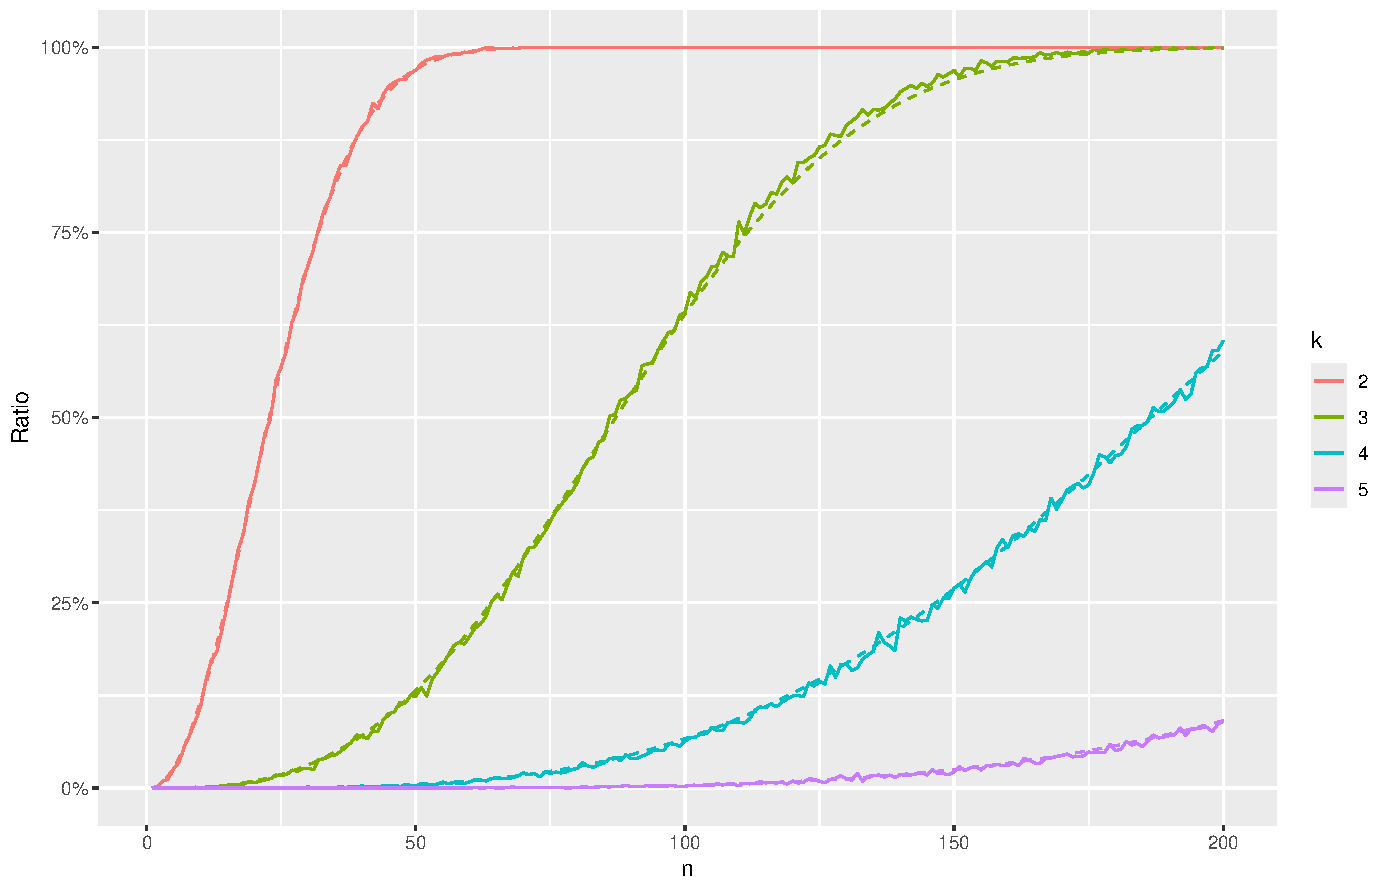
\includegraphics[width=1\textwidth]{src/chapter1/birthday.pdf}
        Here, the lines with dots show the exact theorical ratio. As intended, the lines grealy allign. We can extract whatever information we need from this exact plot. \\
        \end{center}
    \end{enumerate}
\end{enumerate}




